\documentclass[12pt,letterpaper]{article}

\usepackage{tikz}
\usetikzlibrary{shapes}

\usepackage{amssymb,amsmath,amsthm}
\usepackage{enumerate}
\usepackage[margin=1in]{geometry}
\usepackage{graphicx,ctable,booktabs}
\usepackage{fancyhdr}
\usepackage[utf8]{inputenc}
\usepackage{siunitx}

\makeatletter
\newenvironment{problem}{\@startsection
       {section}
       {1}
       {-.2em}
       {-3.5ex plus -1ex minus -.2ex}
       {2.3ex plus .2ex}
       {\pagebreak[3]
       \large\bf\noindent{Problem }
       }
       }
\makeatother

\renewcommand{\thesection}{\Roman{section}}

\title{Quiz $1$: Geometry}
\author{Name: \underline{\hspace{5cm}}
Mark: $\displaystyle \frac{\hspace{3em}}{25}$}
\date{November 21, 2015}

\pagestyle{fancy}
\lhead{Quiz $1$: Geometry}
\chead{}
\rhead{\thepage}
\lfoot{\small\scshape Grade 4 Olympic Math}
\cfoot{}
\rfoot{}
\renewcommand{\headrulewidth}{.3pt}
\renewcommand{\footrulewidth}{.3pt}
\setlength\voffset{-0.25in}
\setlength\textheight{648pt}
\setlength\headheight{15pt}

\newcommand*\circleletter[1]{%
  \begin{tikzpicture}[baseline=(C.base)]
    \node[draw,circle,inner sep=1pt](C) {#1};
  \end{tikzpicture}}

\begin{document}

\maketitle

\thispagestyle{empty}

\noindent\underline{Instructions}

\noindent The test is marked out of $25$. Each part of a question
is worth $2$ marks.

\noindent There are $14$ parts, so there is
$3$-mark bonus available. Note that Problem IV is difficult.

\noindent (Optional) Show work on the scrap paper. Part marks are awarded for
work done.

\noindent All angles that look right are right. All lines
that look parallel are parallel.

\noindent Calculators are permitted but are not needed. Reference formulas on
bottom of back page.

\begin{problem}{Toronto}
\begin{figure}[h]
  \begin{center}
    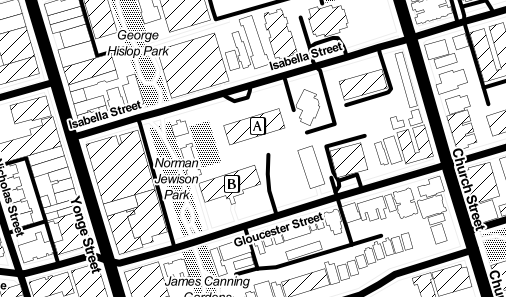
\includegraphics[trim=50 50 50 50, clip, width=.5\textwidth]{toronto.png}
  \end{center}
  \caption{Map from OpenStreetMap}
\end{figure}

 Look at the map of this block in Toronto. Circle the correct response.

 \begin{enumerate}
  \item At what kind of angle do Isabella Street and Yonge Street intersect?

  \hfill Acute~~Right~~Obtuse~~Straight~~Reflex

  \item What kind of shape is Building~\circleletter{A}?
  \hfill Rhombus~~Kite~~Rectangle

  \item What kind of shape is Building~\circleletter{B}?
  \hfill Quadrilateral~~Circle~~Other

  \item What is the sum of interior angles for Building~\circleletter{A}?
  \hfill $90^\circ$~~$180^\circ$~~$360^\circ$~~$540^\circ$

  \item Which building has greater area?
  \hfill Building~\circleletter{A}~~Building~\circleletter{B}
 \end{enumerate}
\end{problem}

\begin{problem}{Triangle}
 A right triangle has base length \SI{10}{\meter}
 and height \SI{10}{\meter}.

 \begin{enumerate}
  \item What is its area?
  \hfill \underline{\hspace{3em}} \si{\meter^2}
  \item How many interior acute angles does the triangle have?
  \hfill \underline{\hspace{3em}}
 \end{enumerate}
\end{problem}

\begin{problem}{Garden}
\begin{figure}[h]
  \begin{center}
    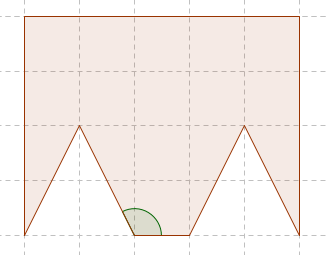
\includegraphics[width=.4\textwidth]{garden.png}
  \end{center}
\end{figure}

 Look at the map of Vegeta's vegetable garden. The shaded part is the
 garden itself. Each grid square represents \SI{1}{\meter^2}. One angle is marked.

 \begin{enumerate}
  \item What kind of angle is the marked angle? (circle one)

  \hfill Acute~~Right~~Obtuse~~Straight~~Reflex

  \item The angle supplementary to the marked angle is $63^\circ$.
  What is the measure of the marked angle?

  \hfill $\underline{\hspace{3em}}^\circ$

  \item How many sides does this garden have? \hfill $\underline{\hspace{3em}}$

  \item How many of the garden's interior angles are reflex angles?
  \hfill $\underline{\hspace{3em}}$

  \item What is the area of this garden? \hfill $\underline{\hspace{3em}}$
  \si{\meter^2}
 \end{enumerate}

\end{problem}

\begin{problem}{Challenge}
 Two angles are complementary. One is $18^\circ$ greater than the other.
 What are the two angles?

 \hfill $\underline{\hspace{3em}}^\circ$, $\underline{\hspace{3em}}^\circ$
\end{problem}

\vspace{1em}\noindent\underline{Reference}

\noindent Area formulas: $A_\Delta=\frac{1}{2}bh$, $A_\square=\ell w$,
$A_\text{parallelogram}=bh$,
$A_\text{trapezoid}=\frac{1}{2}\left(b_1+b_2\right)h$

\noindent Interior angle sum: $\mathrm{AS}=180^\circ (n-2)$

\end{document}
